% Compile with XeLaTeX (not pdfLaTeX).
\documentclass[11pt,a4paper,fontset=fandol]{ctexart}
\usepackage[margin=2.3cm]{geometry}
\usepackage{amsmath,amssymb,booktabs,graphicx}
\usepackage[hidelinks]{hyperref}
\graphicspath{{figures/}}
\setlength{\emergencystretch}{2em}
\title{等变结构是否优于精确增强？\\RQ1、RQ2、RQ3 主实验中文解读}
\author{项目组}
\date{结果冻结日期：2026 年 11 月 23 日}
\begin{document}
\maketitle
% 可复制的中文正文；需要的宏包及插入方法见 README.md。
% 本文用于组内快速理解，不是英文稿的逐句翻译。
\begin{abstract}
这份说明围绕三个问题展开：等变结构是否能帮助 Push-T 减少示范需求；
有了精确旋转增强，等变架构是否还有额外价值；当任务不满足对称性假设时，
这种约束会造成什么损失，以及如何修正。主实验表明，EquiDiff 在
100/200 条示范的固定预算比较中优于普通 DP，但在 25/50 条示范时，
没有充分证据支持稳定的低数据优势。精确增强在 25/50 条示范时更强，
而 200 条示范下的架构优势会随训练加长而缩小。
固定目标且状态输入不含目标时，错误等变约束造成明显性能下降；
显式目标输入与可学习门控可以部分恢复，但仍不及 DP。
因此，我们的结论是等变性具有明确的适用条件，而不是所有原始假设都成立。
以下结论来自已完成的 RQ1、RQ2、RQ3 和补充检查，不依赖可选 E4 的未完成结果。
\end{abstract}

\section{先理解背景：我们究竟在研究什么？}
\label{eqstudy:zh:background}
\subsection{机器人示范学习为什么需要对称性？}
Diffusion Policy（DP）从示范数据学习：看到当前场景后，应该生成怎样的动作序列。
它通过扩散去噪来表达复杂的动作分布，再执行部分动作、重新观察并继续控制
\cite{chi2023diffusion}。这种方法有效，但示范采集通常昂贵。

一个直观例子是：机器人已经学会从一个方向推动物体，如果把场景整体转
$90^\circ$，理想的策略应该把动作也转 $90^\circ$，而不是重新学习一遍。
这里的规律叫作旋转等变性。

\subsection{架构等变与数据增强有什么区别？}
普通 DP 不强制满足旋转规律。DP 加旋转增强把图像、位置和动作标签一起旋转，
让网络从更多方向的训练样本中学习规律。EquiDiff 则通过等变特征与参数共享，
把旋转关系写进网络结构\cite{wang2024equivariant}。

去噪函数的等变关系可写为
\begin{equation}
\epsilon_\theta(g o,g a_k,k)=g\epsilon_\theta(o,a_k,k),
\label{eqstudy:zh:equivariance}
\end{equation}
其中 $o$ 是观测，$a_k$ 是带噪动作，$g$ 是旋转。直观地说，就是输入一起转，
预测的噪声也按同样规则转。对于随机策略，这种关系主要针对动作分布，
不要求两次使用独立随机噪声的采样轨迹完全一样。

我们的工作不是重新证明 EquiDiff 的定理，而是检验它在新的任务和条件下是否有效。
主实验是 EquiDiff 核心架构的 Push-T 适配，不是项目早期的 Frame Averaging 备选实现。

\section{Research Gap：为什么还需要我们的实验？}
\label{eqstudy:zh:gap}
\paragraph{缺口一：换一个任务家族，低数据优势还成立吗？}
原论文主要研究三维桌面操作；我们研究二维接触推动 Push-T。
操作形式、动作表示和接触过程不同，所以原论文的优势不能直接搬到这里。
这对应 RQ1。

\paragraph{缺口二：之前比较的是架构，还是增强质量？}
在斜视角图像上做二维旋转，通常不等于把真实三维场景旋转。
如果增强样本与物理动作不一致，增强基线可能受到额外影响。
我们选择可以构造精确 $90^\circ$ 变换的场景，重新比较架构与增强。
这对应 RQ2。它不意味着我们已经证明原论文所有增强样本都错误，
也不意味着可以用 Push-T 分数否定原论文结果。

\paragraph{缺口三：如果对称性假设错了，会不会越约束越差？}
目标若固定在世界坐标中，而网络看不到目标，却被要求对状态旋转保持等变，
网络可能无法表达任务所需的固定方向偏好。
我们需要测量这种损失，并尝试恢复性能。这对应 RQ3。

\section{共同实验设置与读数方法}
\label{eqstudy:zh:protocol}
\subsection{Push-T、C4 与数据量}
Push-T 要求一个平面 agent 推动 T 形块，使其与目标形状对齐。
$C_4$ 表示四种旋转：$0^\circ$、$90^\circ$、$180^\circ$ 和 $270^\circ$。
正方形边界与像素格点对这些旋转兼容，图像可以直接用无插值的
\texttt{rot90} 处理。

实际旋转中心是 $(255.5,255.5)$，原目标位置 $(256,256)$ 连同朝向一起旋转。
四个目标位置因此是 $(256,256)$、$(256,255)$、$(255,255)$ 和 $(255,256)$。
这修正了 proposal 中只描述目标角度变化的简化说法。

物理在各个旋转坐标系中原生运行；渲染把状态逆变换到规范场景，调用原始渲染器，
再做精确像素旋转。规范场景仅用于渲染，不推进额外物理。
因此，像素等变性来自明确构造，不能说原始相机或渲染器天然精确等变。
留出示范的原生回放验证中，最大位置误差约 $4.89\times10^{-11}$，
coverage 误差约 $1.20\times10^{-12}$；构造渲染的旋转像素误差为零。
这些是所测配置下的验证，不是所有可能状态上的证明。

官方数据共 206 条示范，其中 200 条用于训练，6 条留出验证。
主实验采用嵌套的 25、50、100、200 条训练子集。
旋转增强不会把一条独立示范变成多条独立示范。
各方法共享轨迹身份和尽量平衡的固定基础朝向；只有增强方法额外做在线旋转。

\subsection{什么叫公平预算？}
主图像实验统一为 20,000 次优化更新、batch 64、AdamW、学习率 $10^{-4}$、
U-Net 宽度 $[512,1024,2048]$、EMA，以及 100 步扩散训练和推理。
观测历史长度为 2，预测动作序列长度为 16，每次执行 8 步；使用 FP32，禁用 TF32。

我们控制的是更新次数，而不是相同运行时间或完全相同参数量。
EquiDiff-C4 约 257.6M 参数，DP 约 288.4M。
三个训练 seed（0、1、2）代表三次独立随机训练；同一个模型多测几次，
不能算作增加了训练 seed。

\subsection{Coverage 不是成功率，也不是 IoU}
单步覆盖程度为
\begin{equation}
c_t=\frac{\operatorname{area}(\text{物体}_t\cap\text{目标})}
{\operatorname{area}(\text{目标})}.
\label{eqstudy:zh:coverage}
\end{equation}
每个 episode 最多运行 300 个控制步，分数取过程中的最大 coverage。
只有 coverage 严格大于 $0.95$ 才算成功。
因此 coverage 为 $0.67$ 不等于成功率为 $67\%$。

每个 checkpoint 在 25 个预留基础初态及其四个朝向上评估，共 100 episodes。
主指标对 16k、18k、20k 三个预先保留的 EMA checkpoint 求平均，
再汇总测试初态和三个训练 seed。
这不是单独 20k checkpoint 的分数，也不是训练全程最高分。

表中 ``$\pm$'' 是三个 seed 的样本标准差。
差值的 95\% 置信区间采用 10,000 次配对 bootstrap，
同时重采样训练 seed 和基础初态，并保留同一初态四个朝向的配对关系。
区间包含零表示现有证据不能确定差异方向，不能解释为两种方法已经被证明相等。
只有三个训练 seed，且多个比较未做多重比较校正，结论需要保留这些限制。

\section{RQ1：等变结构的数据效率能否迁移到 Push-T？}
\label{eqstudy:zh:rq1}
\subsection{问题与目的}
我们想知道：如果只给较少的示范，EquiDiff 能否比普通 DP 学得更好？
原 proposal 的 H1 预测，在不超过 50 条示范时 EquiDiff 应该占优。
这里检验的是跨任务的数据效率，不是复现原论文的 MimicGen 数值。

\subsection{实验设计}
使用 25/50/100/200 条示范，比较 DP、DP 加精确增强、EquiDiff-C4，
每组训练三个 seed。共 $4\times3\times3=36$ 次训练。
RQ1 主要看 EquiDiff 与 DP 的差别；RQ2 使用同一批实验中的增强基线，
不重复计算训练数量。

\subsection{实验结果}
\begin{table}[htbp]
\centering
\caption{主图像实验 coverage：三个 seed 均值及标准差。粗体仅标记最高均值。}
\label{eqstudy:zh:tab:main}
\resizebox{\linewidth}{!}{%
\begin{tabular}{rccc}
\toprule
示范数 & DP & DP + 精确增强 & EquiDiff-C4 \\
\midrule
25 & $0.2076\pm0.0126$ & $\mathbf{0.4598}\pm0.0604$ & $0.1893\pm0.0236$ \\
50 & $0.2899\pm0.0385$ & $\mathbf{0.5787}\pm0.0104$ & $0.3465\pm0.0173$ \\
100 & $0.4675\pm0.0460$ & $\mathbf{0.6166}\pm0.0194$ & $0.5789\pm0.0277$ \\
200 & $0.5721\pm0.0276$ & $0.5828\pm0.0074$ & $\mathbf{0.6712}\pm0.0518$ \\
\bottomrule
\end{tabular}}
\end{table}

\begin{table}[htbp]
\centering
\caption{RQ1：EquiDiff-C4 减 DP 的 coverage 差值。}
\label{eqstudy:zh:tab:rq1}
\begin{tabular}{rcl}
\toprule
示范数 & 差值 & 配对 95\% 置信区间 \\
\midrule
25 & $-0.0183$ & $[-0.0597,\;0.0262]$ \\
50 & $+0.0565$ & $[-0.0220,\;0.1391]$ \\
100 & $+0.1115$ & $[0.0279,\;0.1896]$ \\
200 & $+0.0991$ & $[0.0247,\;0.1596]$ \\
\bottomrule
\end{tabular}
\end{table}

\begin{figure}[htbp]
\centering
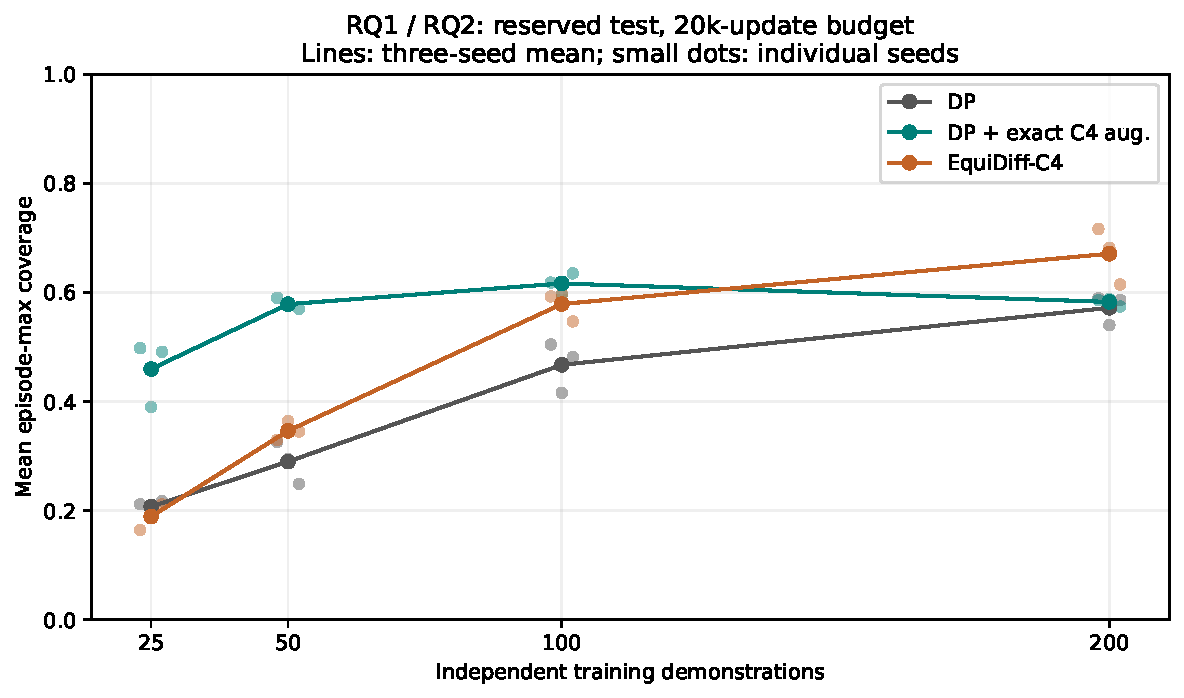
\includegraphics[width=0.9\linewidth]{rq1_rq2_test.pdf}
\caption{RQ1/RQ2 主测试曲线。线表示均值，小点表示各训练 seed。}
\label{eqstudy:zh:fig:main}
\end{figure}

\subsection{结果分析}
25 条示范时，EquiDiff 的均值甚至略低于 DP；50 条时均值更高，
但置信区间仍跨零，因此不能把这个均值优势说成稳定结论。
100 和 200 条时，差值区间不包含零，支持本协议下 EquiDiff 更好。
这说明结构可以迁移，但收益并没有首先出现在我们原先最期待的极低数据条件。

\subsection{结论与汇报说法}
\textbf{H1 未获支持。} 可以说：
``EquiDiff 在中高示范数量下优于 DP，但低数据优势没有稳定迁移到当前 Push-T 协议。''
不应说：``等变结构已经证明在任何少样本条件下更好。''
优化难度和数据分布都可能影响结果，但这些可能原因没有被逐项隔离验证。

\section{RQ2：有了精确增强，还需要等变架构吗？}
\label{eqstudy:zh:rq2}
\subsection{问题与目的}
只和无增强 DP 比较，不能回答架构是否有不可替代的价值。
我们要问：如果普通 DP 也得到物理正确的旋转训练样本，架构还能多带来多少收益？
原 H2 预测，相对精确增强的优势会缩小，可能不再明显。

\subsection{实验设计}
直接复用表~\ref{eqstudy:zh:tab:main} 的 36 次训练，比较增强方法与 EquiDiff。
增强只使用精确 $C_4$ 变换，图像和几何标签保持一致；
不引入 45 度插值旋转，也不增加独立示范条数。

\subsection{实验结果}
\begin{table}[htbp]
\centering
\caption{RQ2：EquiDiff-C4 减 DP + 精确增强的 coverage 差值。}
\label{eqstudy:zh:tab:rq2}
\begin{tabular}{rcl}
\toprule
示范数 & 差值 & 配对 95\% 置信区间 \\
\midrule
25 & $-0.2705$ & $[-0.3597,\;-0.1871]$ \\
50 & $-0.2322$ & $[-0.3118,\;-0.1512]$ \\
100 & $-0.0377$ & $[-0.1145,\;0.0260]$ \\
200 & $+0.0884$ & $[0.0193,\;0.1452]$ \\
\bottomrule
\end{tabular}
\end{table}

\subsection{结果分析}
25 和 50 条示范时，精确增强明显优于 EquiDiff；100 条时增强均值更高，
但差异不确定；200 条时，EquiDiff 在当前训练预算内占优。
因此，精确增强不是一个可以忽略的弱基线。

我们另做了三种方法在四个数据量、各三个 seed 下的独立收敛检查，
共 36 次训练，比较 20k、40k、60k 的验证分数。
这些是\textbf{独立验证曲线}，不能与主测试表混作同一条学习曲线。
增强与 EquiDiff 的补充检查是在看到主结果后安排，具有探索性。

\begin{table}[htbp]
\centering
\caption{独立验证集上 20k $\rightarrow$ 60k 更新的 coverage。每条曲线含三个 seed。}
\label{eqstudy:zh:tab:conv}
\resizebox{\linewidth}{!}{%
\begin{tabular}{rccc}
\toprule
示范数 & DP & DP + 精确增强 & EquiDiff-C4 \\
\midrule
25 & $0.1646\to0.1661$ & $0.4215\to0.4700$ & $0.1716\to0.1945$ \\
50 & $0.2254\to0.2310$ & $0.6278\to0.6377$ & $0.3181\to0.4053$ \\
100 & $0.4372\to0.4551$ & $0.6472\to0.7702$ & $0.5322\to0.6260$ \\
200 & $0.5765\to0.5964$ & $0.5751\to0.7422$ & $0.6386\to0.7501$ \\
\bottomrule
\end{tabular}}
\end{table}

\begin{figure}[htbp]
\centering
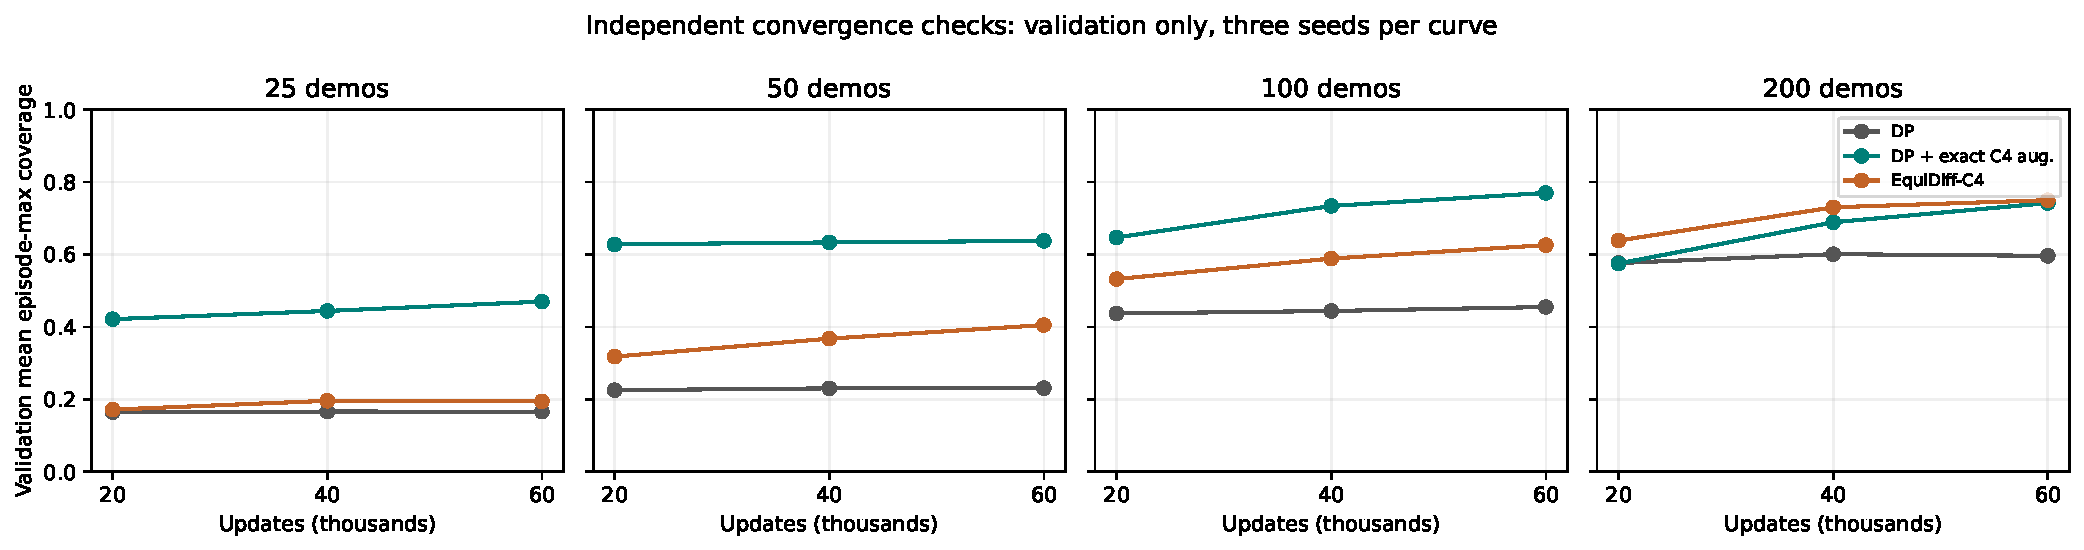
\includegraphics[width=\linewidth]{convergence_validation.pdf}
\caption{独立验证收敛检查；不是主实验测试集结果的延长或替换。}
\label{eqstudy:zh:fig:conv}
\end{figure}

特别是在 200 条示范时，EquiDiff 与增强的验证均值差距从约 $0.0634$
缩小到约 $0.0080$。这提示主实验优势与预算有关，不能当作更高最终性能上限的证明。
两者接近也不等于已经证明等价，60k 并不保证充分收敛。

\subsection{结论与汇报说法}
\textbf{H2 的方向性动机得到支持，但不是所有条件都没有差异。}
可以说：``精确增强在少数据条件下更有效，结构优势取决于示范数量和训练预算。''
不能把我们的 coverage 差值与原论文的成功率差值直接相减，
从而宣称定量复现或推翻了原论文 Appendix I。

\paragraph{补充：C8 消融。}
50/200 条示范时，C8 分别为 $0.2903/0.5826$，低于 C4 的 $0.3465/0.6712$。
C4 减 C8 的差值区间分别为 $[0.0151,0.1048]$ 和 $[0.0223,0.1621]$。
但当前墙体、像素格点并不具有精确 45 度对称性，DDPM 逐坐标 clipping
也只与 C4 兼容；参数量及运行环境还有差异。
所以它是架构消融，不能推出``旋转群越大越差''这一普遍结论。

\section{RQ3：错误对称性有多大危害，修正能恢复多少？}
\label{eqstudy:zh:rq3}
\subsection{问题与目的}
考虑目标始终固定在世界坐标中的任务。如果网络只看到 agent 和物体状态，
又被强制要求``场景一转，动作也必须同样转''，这个约束可能与固定目标冲突。
RQ3 要检验这种损失，并检验能否恢复。
H3 包含两个独立预测：普通 EquiDiff 会比 DP 差；加入目标后能恢复到至少 DP 水平。

\subsection{实验设计}
主要机制实验使用状态输入：agent 位置、物体位置、物体朝向；
普通模型不含目标。设置固定目标和旋转目标两种条件，四种模型各三个 seed，
共 $2\times4\times3=24$ 次训练。每次 50 条示范、20k 更新、batch 64，
状态 U-Net 宽度为 $[128,256,512]$，不与图像模型跨模态排名。

四种模型分别是：
\begin{enumerate}
\item \textbf{DP：}不强制旋转等变，可以学到固定的世界方向偏好。
\item \textbf{EquiDiff：}对普通状态输入施加等变约束，作为失效研究对象。
\item \textbf{EquiDiff + goal：}把目标朝向作为额外向量输入，让模型得到任务参照。
该朝向也决定当前 C4 轨道中的目标亚像素位置偏移。
\item \textbf{EquiDiff + gate：}加入固定世界向量 $(1,0)$，乘以零初始化的可学习标量。
开始时保持等变，训练可以学习偏离严格等变。
这一思路参考近似等变模型的动机\cite{wang2022approximately}，并非对其完整方法的复现。
\end{enumerate}

注意：固定目标即使没有输入，DP 仍可从训练中学到这个常量目标。
因此问题不是``没输入目标就一定无法完成''，而是模型约束是否允许它表达正确映射。
旋转目标下，普通状态模型仍然缺少目标信息，不能认为其任务已经完全可观测。

\subsection{实验结果}
\begin{table}[htbp]
\centering
\caption{RQ3 状态输入的主 coverage，均值及 seed 标准差。}
\label{eqstudy:zh:tab:state}
\resizebox{\linewidth}{!}{%
\begin{tabular}{lcccc}
\toprule
条件 & DP & EquiDiff & EquiDiff + goal & EquiDiff + gate \\
\midrule
固定目标 & $\mathbf{0.7869}\pm0.0270$ & $0.4888\pm0.0232$ & $0.6183\pm0.0340$ & $0.6223\pm0.0075$ \\
旋转目标 & $0.4061\pm0.0123$ & $0.4733\pm0.0340$ & $\mathbf{0.5584}\pm0.0085$ & $0.4771\pm0.0492$ \\
\bottomrule
\end{tabular}}
\end{table}

\begin{figure}[htbp]
\centering
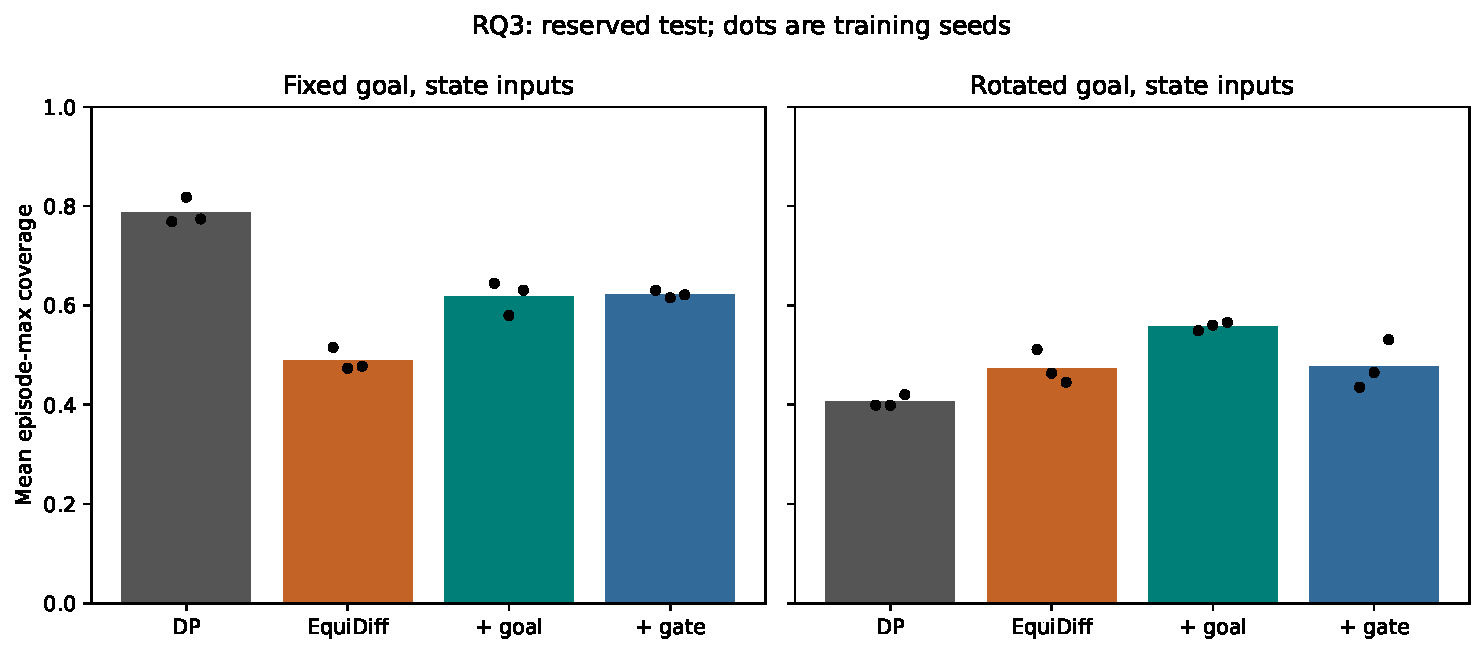
\includegraphics[width=\linewidth]{rq3_state_test.pdf}
\caption{RQ3 状态实验：固定目标下出现明显损失，两种修正均部分恢复。小点为各训练 seed。}
\label{eqstudy:zh:fig:state}
\end{figure}

\begin{table}[htbp]
\centering
\caption{固定目标状态实验的关键差值。}
\label{eqstudy:zh:tab:repair}
\begin{tabular}{lcl}
\toprule
比较方向 & coverage 差值 & 95\% 置信区间 \\
\midrule
EquiDiff $-$ DP & $-0.2981$ & $[-0.3676,-0.2282]$ \\
goal $-$ EquiDiff & $+0.1295$ & $[0.0631,0.1915]$ \\
gate $-$ EquiDiff & $+0.1335$ & $[0.0732,0.1938]$ \\
goal $-$ DP & $-0.1686$ & $[-0.2448,-0.0932]$ \\
gate $-$ DP & $-0.1646$ & $[-0.2248,-0.1070]$ \\
gate $-$ goal & $+0.0039$ & $[-0.0543,0.0570]$ \\
\bottomrule
\end{tabular}
\end{table}

\subsection{结果分析}
固定目标下，错误等变约束使 coverage 从 DP 的 $0.7869$ 降到 $0.4888$。
两种修正都恢复约 $0.13$，但恢复后的 $0.6183/0.6223$ 仍明显低于 DP。
goal 和 gate 之间的区间跨零，不能宣布其中一种修正更好。

旋转目标下 goal-input 均值最高，但不能仅凭均值排名就认为所有差异都可靠。
普通 EquiDiff 减 DP 的 coverage 区间为 $[-0.0149,0.1462]$；
goal 减 DP 的区间为 $[0.0416,0.2582]$；goal 与普通 EquiDiff 的区间仍跨零。
目标输入同时增加信息与参照，因此收益不是单纯隔离出来的架构效应。

\subsection{结论与汇报说法}
\textbf{H3 部分成立。} ``错误约束有害''得到支持；
``目标输入恢复到至少 DP 水平''没有得到支持。
可以说：``两种修正均有效地恢复了部分性能，但没有完全消除损失。''
不能说：``我们已经解决了错误等变性问题。''

\subsection{补充检查：如果图像已经显示目标呢？}
图像扩展比较固定/旋转目标下的 DP、C4、C4 + gate，共 18 个比较单元。
其中 6 个旋转目标基线复用 RQ1，实际新增 12 次训练。
因为图像已经包含目标，没有再增加显式 goal-input 图像臂。
该扩展在观察早期结果后设计，属于探索性。

\begin{table}[htbp]
\centering
\caption{目标可见的图像扩展：主 coverage 均值。}
\label{eqstudy:zh:tab:image}
\begin{tabular}{lccc}
\toprule
条件 & DP & EquiDiff-C4 & C4 + gate \\
\midrule
固定目标 & 0.3241 & 0.3348 & 0.3087 \\
旋转目标 & 0.2899 & 0.3465 & 0.3225 \\
\bottomrule
\end{tabular}
\end{table}

固定图像条件中，C4 减 DP 的 coverage 区间为 $[-0.0653,0.0876]$，
没有出现状态实验中同样的大幅下降。gate 与 C4 的区间在两种图像条件下都跨零。
这并不矛盾，因为图像中的目标提供了普通状态输入没有的参照。
不能把它当作隐藏目标机制的第二次独立确认，也不能把图像与状态结果混在一起。

\section{辅助读数：成功率与假设判定}
\label{eqstudy:zh:conclusions}
\begin{table}[htbp]
\centering
\caption{主图像实验的平均成功率，阈值为 coverage $>0.95$。}
\label{eqstudy:zh:tab:success}
\begin{tabular}{rccc}
\toprule
示范数 & DP & DP + 精确增强 & EquiDiff-C4 \\
\midrule
25 & 0.11\% & 2.00\% & 0.33\% \\
50 & 1.00\% & 3.78\% & 2.33\% \\
100 & 1.33\% & 1.11\% & 5.89\% \\
200 & 2.67\% & 0.78\% & 11.89\% \\
\bottomrule
\end{tabular}
\end{table}

这些成功率仍然不高，说明我们完成的是固定预算下的相对性能研究，
不是已经得到可靠部署策略。固定目标状态实验中，DP、EquiDiff、goal、gate
成功率分别为 $34.89\%$、$5.67\%$、$17.00\%$、$18.89\%$，
与部分恢复的方向一致。固定目标图像中，DP 与 C4 成功率分别为 $6.44\%$ 和 $1.33\%$，
因此 coverage 相近也不能表述成成功率相同。

对原始预测可以逐条回答：
\begin{itemize}
\item H1：低数据时 EquiDiff 稳定优于 DP，\textbf{未获支持}。
\item H2：精确增强会削弱架构的普遍优势，\textbf{方向性支持，但取决于数据量与预算}。
\item H3 的失效部分：错误等变性有害，\textbf{获支持}。
\item H3 的完全恢复部分：goal 达到或超过 DP，\textbf{未获支持}。
\end{itemize}

\section{E4 与三个主问题的关系}
\label{eqstudy:zh:e4}
\textbf{E4 在原 proposal 中，但明确属于可选扩展，不是 RQ1/RQ2/RQ3 的缺失部分。}
原文写的是：
\begin{quote}
\emph{Optional E4}: train the 6-DoF EquiDiff and DP on MimicGen D0 and test on D1/D2,
a quantitative version of the paper's qualitative App. M.
\end{quote}
原文还写了 ``MimicGen datasets for E4 only''，并在计算预算不足时允许 ``drop E4''。

它回答的是：在 MimicGen 的 D0 分布训练后，能否不微调地迁移到更难的 D1/D2。
本次实现选用 Square 任务家族，不覆盖全部 MimicGen 任务。
它归档在 RQ1 的目录下，是为了按迁移主题组织文件，不代表它是 RQ1 主矩阵的一部分。

截至本报告冻结时，E4 的最终迁移评估尚未完成。
我们没有用其中途 D0 分数支持 D1/D2 结论，主报告也不需要等待它才能形成结论。

\section{范围、限制与组内汇报用结论}
\label{eqstudy:zh:limits}
\subsection{实验完成范围}
本报告包含 RQ1/RQ2 共享主矩阵 36 次、RQ3 状态 24 次、C8 消融 6 次、
RQ3 图像新增 12 次、独立收敛检查 36 次，共 114 次独立训练。
其中 78 次用于主测试和扩展测试，36 次用于独立验证。
每次三个 checkpoint、每个 100 episodes，共 34,200 条评估记录，
这些是重复测量，不是 34,200 个独立统计样本。
预检、早期 pilot、单 seed 官方参考以及未完成 E4 均不计入该数量。

\subsection{需要保留的限制}
证据来自一个 Push-T 任务家族、三个训练 seed 和有限初态。
20k 更新不代表充分收敛，60k 也不代表性能上限。
不同方法不完全匹配参数量与运行成本，补充实验还跨不同 GPU 和 PyTorch 版本。
精确 C4 渲染构造不能直接外推到真实相机的连续旋转。
目标输入改变可用信息，门控改变函数类；因此机制解释仍有信息与优化上的混杂因素。
有限三个 checkpoint 的最高分也不等于原论文完整训练过程的最高分。

\subsection{可以直接用于汇报的一段话}
我们在具有可控 C4 对称性的 Push-T 平台上，比较了普通扩散策略、精确数据增强和等变架构。
结果表明，等变结构的收益取决于数据量和训练预算：它在中高数据量的固定预算比较中优于 DP，
但低数据量优势没有稳定出现，精确增强反而在 25/50 条示范时更有效。
错误对称性约束会造成明显损失，目标信息和可学习对称性破坏能部分恢复，但没有完全恢复到 DP 水平。
因此，是否采用等变结构，需要同时考虑任务对称性、目标可观测性和训练预算。
原假设没有全部成立，但三个研究问题已经有明确的实验回答。

\bibliographystyle{plain}
\bibliography{references}
\end{document}
